\documentclass[12pt,a4paper]{article}
\usepackage[utf8]{inputenc}
\usepackage{mathtools}
\usepackage{amssymb}
\usepackage[norsk]{babel}
\usepackage{graphicx}
\usepackage{tikz}

\usepackage{listings}
\usepackage{color}
\usetikzlibrary{trees}


\newcommand{\intt}{integritetsregler}
\newcommand{\inttt}{integritetsregel}
\newcommand{\Intt}{Integritetsregler}
 
\definecolor{dkgreen}{rgb}{0,0.6,0}
\definecolor{gray}{rgb}{0.5,0.5,0.5}
\definecolor{mauve}{rgb}{0.58,0,0.82}


\lstset{ %
  language=sql,                % the language of the code
  basicstyle=\small,           % the size of the fonts that are used for the code
  numbers=left,                   % where to put the line-numbers
  numberstyle=\small\color{gray},  % the style that is used for the line-numbers
  stepnumber=1,                   % the step between two line-numbers. If it's 1, each line 
                                  % will be numbered
  numbersep=5pt,                  % how far the line-numbers are from the code
  backgroundcolor=\color{white},      % choose the background color. You must add \usepackage{color}
  showspaces=false,               % show spaces adding particular underscores
  showstringspaces=false,         % underline spaces within strings
  showtabs=false,                 % show tabs within strings adding particular underscores
  frame=none,                   % adds a frame around the code
  rulecolor=\color{black},        % if not set, the frame-color may be changed on line-breaks within not-black text (e.g. commens (green here))
  tabsize=2,                      % sets default tabsize to 2 spaces
  captionpos=b,                   % sets the caption-position to bottom
  breaklines=true,                % sets automatic line breaking
  breakatwhitespace=false,        % sets if automatic breaks should only happen at whitespace
  title=\lstname,                   % show the filename of files included with \lstinputlisting;
                                  % also try caption instead of title
  keywordstyle=\color{blue},          % keyword style
  commentstyle=\color{dkgreen},       % comment style
  stringstyle=\color{mauve},         % string literal style
  escapeinside={\%*}{*)},            % if you want to add LaTeX within your code
  morekeywords={*,...}               % if you want to add more keywords to the set
}

\title{Notater: INF3100}
\author{Veronika Heimsbakk \\ 
veronahe@student.matnat.uio.no}
\begin{document}

\maketitle{}
\tableofcontents
\newpage{}

\section{Intro}
Disse notatene er basert på egne notater og forelesningsfoilene til Ellen Munthe-Kaas fra \textit{INF3100 - Databasesystemer} våren 2013, notatene er i meget liten grad basert på pensumboka. Notatene inneholder sikkert veldig mange skrivefeil, uten at dette skal gå ut over innholdet. Merk også at det finnes noen mangler, dette inkluderer bl.a. bagoperasjoner, theta-join, ekvijoin og divisjon.

\section{Relasjonsdatabasedesign}
\subsection{Funksjonelle avhengigheter}
$X \rightarrow Y$, $Y$ følger av $X$.

\begin{itemize}
\item{Refleksiv: hvis $Y \subseteq X$, så $X \rightarrow Y$}
\item{Utvidelse: hvis $X \rightarrow Y$, så $XZ \rightarrow YZ$}
\item{Transitiv: hvis $X \rightarrow Y$ og $Y \rightarrow Z$, så $X \rightarrow Z$}
\end{itemize}

En refleksiv FD kales triviell fordi den automatisk er oppfylt.

\paragraph{Ekvivalente mengder av FDer} Hvis $X$ er en supernøkkel, så holder $X \rightarrow Y$ for alle $Y$.
$Y$ er like sterk, eller sterkere enn $X$. Ekvivalente. $X$ følger av $Y$ og $Y$ følger av $X$.

Hvis det fins et attributt som ikke fins i høyresiden til noen FD, så må den være med i \textit{alle} kandidatnøklene.

\paragraph{Eksempel}
Gitt $F = \{AB \rightarrow DE, C \rightarrow A, BD \rightarrow E, AE \rightarrow B\}$ på relasjonen $R(A, B, C, D, E)$. Her må $C$ være med i alle kandidatnøklene.

$C^{+} = AC$, så $C$ er ingen supernøkkel.
$BC^{+} = ABCDE$, så dette er en kandidatnøkkel. Det samme er $CE^{+}$. $BC$ og $CE$ er de eneste kandidatnøklene i $R$.

\subsubsection{Trivielle FDer}
En FD som følger av refleksivitetsregelen: «Hvis Y er en delmengde av X, så X $\rightarrow$ Y» kalles \textit{triviell} fordi den er automatisk oppfylt. En FD X $\rightarrow$ Y hvor Y $-$ X $\neq \emptyset$, kalles \textit{ikke-triviell}. 

\subsubsection{Elementære FDer}
En FD $X \rightarrow A$ kalles elementær dersom
\begin{itemize}
\item{$A$ er et attributt.}
\item{$X \rightarrow A$ er ikke-triviell.}
\item{$X$ er minimal (dvs. at hvis $X \subseteq Y$ og $Y \rightarrow A$, så $Y = X$.}
\end{itemize}

En kandidatnøkkel $K$ er elementær hvis det finnes en elementær FD $K \rightarrow B$ i $R$. Iallefall ett attributt $B$ som avhenger av hele $K$.

\subsection{Hvordan finne kandidatnøkler}
Gitt F = \{AB $\rightarrow$ DE, C $\rightarrow$ A, BD $\rightarrow$ E, AE $\rightarrow$ B\} på relasjonen R(A, B, C, D, E).
\begin{description}
\item[] Ettersom C ikke er med i noen høyreside av FDene, må C være med i alle kandidatnøkler.
\item[C$^+$ = AC] C alene er ingen supernøkkel.
\item[BC$^+$ = ABCDE] er en kandidatnøkkel, siden vi får tak i alle attributter ved å gå fra BC.
\item[CE$^+$ = ABCDE] er også en kandidatnøkkel.
\end{description}

BC og CE er de eneste kandidatnøklene til R.

\subsection{Dekomposisjon}
Gitt en relasjon $R(A_1, A_2, \ldots, A_n)$. En dekomposisjon $D = \{R_1, \ldots, R_m\}$ av $R$. 
\begin{enumerate}
\item{Alle attributter i hver $R_k$ er også attributt i $R$.}
\item{Samtlige attributter $A_1, \ldots, A_n$ kan gjenfinnes i minst en av relasjonene $R_1, \ldots, R_m$.}
\end{enumerate}

De samme egenskapene skal bli med i dekomposisjonen. Dekomposisjonen er \textit{tapsfri}, dvs. natural join aldri vil gi falske tupler.
Problemer ved dekomposisjon kan være hvordan vurdere objektivt om en samling relasjoner er god/dårlig? Og hvordan sikre at den aldri gir falske tupler? 

\subsection{Natural join}
\begin{itemize}
\item{Ønsker å kunne rekonstruere den opprinnelige ekstensjonen.}
\item{Slår sammen tupler hvis og bare hvis de har like verdier i attributter med likt kolonnenavn.}
\end{itemize}

\paragraph{Eksempel}
Gitt tabellene: \textsf{Kunde(knr, navn, adr)} og \textsf{Ordre(kode, knr, \#bestilt)}. 

\begin{figure}[h!]
	\centering
		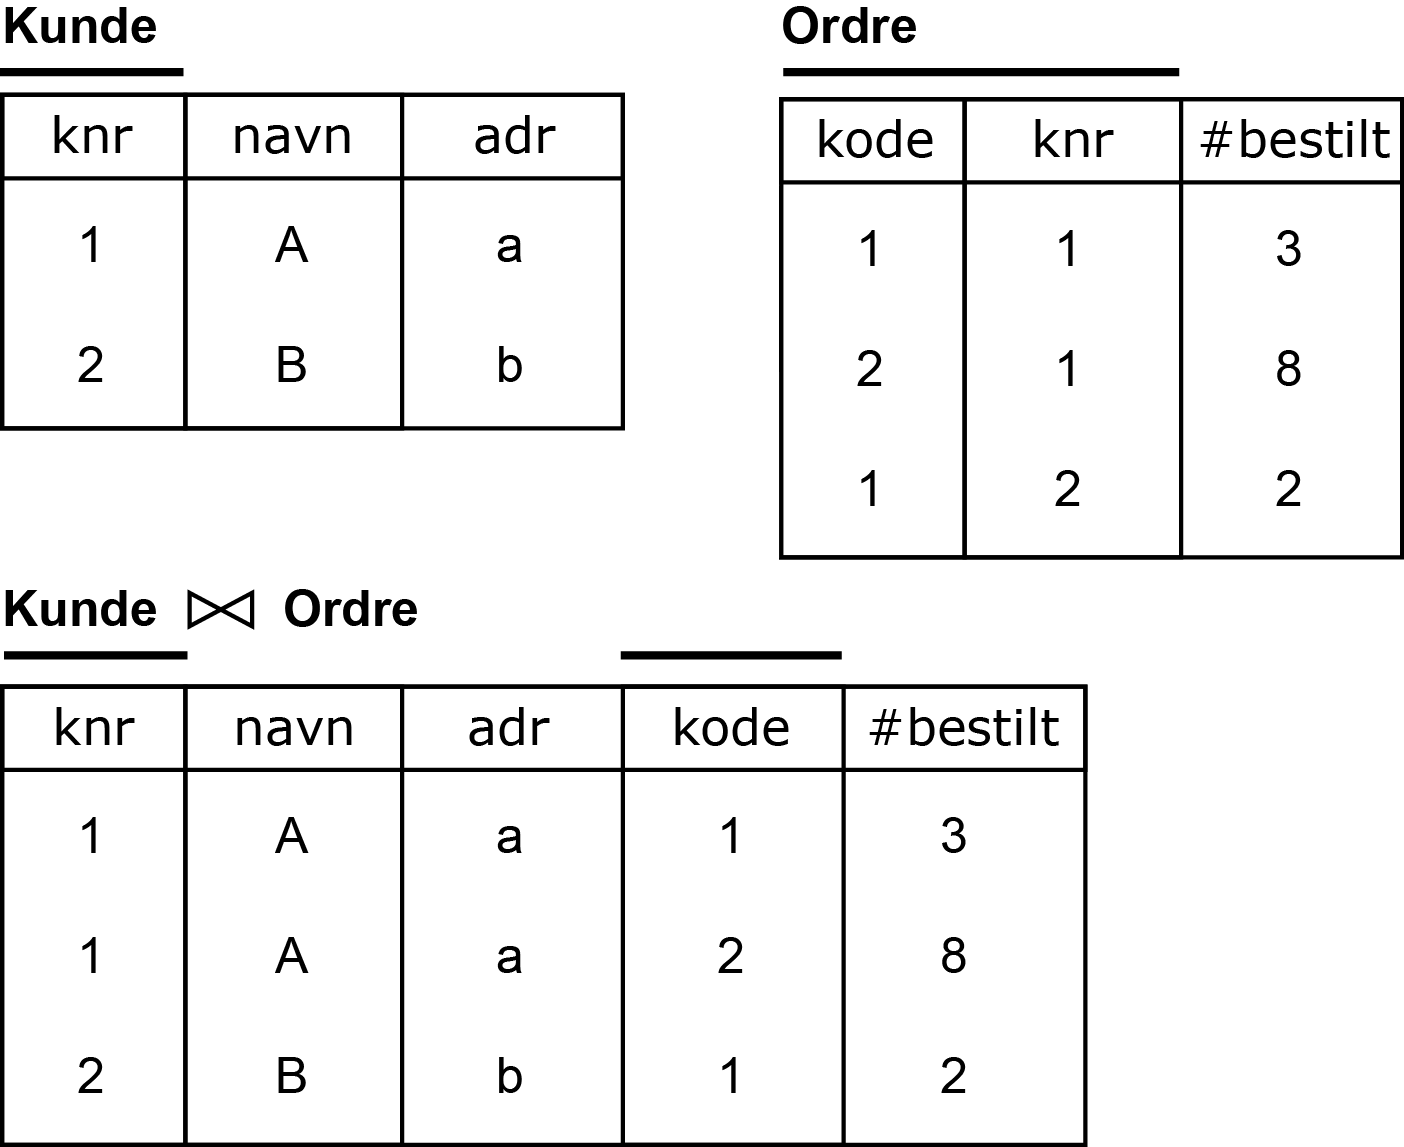
\includegraphics[width=250px]{img/eks1.png}
	\caption{Eksempel på natural join.}
\end{figure}

\section{Normalformer}

Normalformer (NF) brukes til å vurdere når man skal dekomponere.

\begin{figure}[h!]
	\centering
		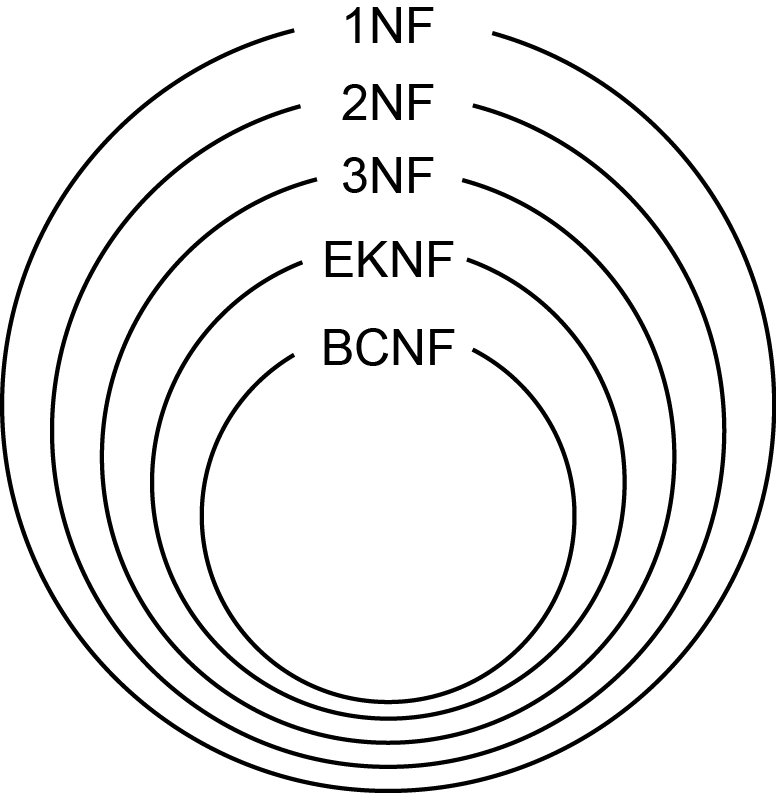
\includegraphics[width=150px]{img/nf.png}
	\caption{Normalformene fra 1NF til BCNF. EKNF er kursorisk pensum for INF3100.}
\end{figure}

Felles for alle normalformene i Fig. 2 er at alle integritetsregler er i form av FDer. Når en normalform brytes skal man dekomponere ved å bruke fagins teorem.

\paragraph{Første normalform - 1NF} alle domenene består av atomære verdier. Alle relasjoner er automatisk 1NF.

\paragraph{Andre normalform - 2NF} En relasjon $R$ er på 2NF hvis \textit{alle} ikke-trivielle FDer i $R$ på formen $X \rightarrow A$, der $X$ er mengden attributter og $A$ er et attributtt i $R$, som tilfredsstiller \textit{minst ett} av følgende krav:
\begin{enumerate}
\item{$X$ er en kandidatnøkkel i $R$ eller inneholder en.}
\item{$A$ er med i en kandidatnøkkel.}
\item{Det er ingen kandidatnøkkel som inneholder $X$.}
\end{enumerate}

\paragraph{Tredje normalform - 3NF} $R$ er på 3NF hvis \textit{alle} ikke-triville FDer i $R$ på formen $X \rightarrow A$ tilfredsstiller \textit{minst ett} av følgende:
\begin{enumerate}
\item{$X$ er en kandidatnøkkel i $R$ eller inneholder en.}
\item{$A$ er med i en kandidatnøkkel.}
\end{enumerate}

3NF $\subseteq$ 2NF, men skjerping av krav i 3NF. 3NF er også lett å oppnå.

\paragraph{Elementary Key Normal Form - EKNF} $R$ er på EKNF hvis \textit{alle} ikke-trivielle FDer i $R$ på formen $X \rightarrow A$ oppfyller \textit{minst ett} av følgende:
\begin{enumerate}
\item{$X$ er en supernøkkel i $R$.}
\item{$A$ er et attributt i en elementær kandidatnøkkel i $R$.}
\end{enumerate}

EKNF $\subseteq$ 3NF, med skjerping av krav fra 3NF.

\paragraph{Boyce-Codd Normal Form - BCNF} $R$ er BCNF hvis \textit{alle} ikke-trivielle FDer i $R$ på formen $X \rightarrow A$ oppfyller:
\begin{enumerate}
\item{$X$ er en supernøkkel i $R$.}
\end{enumerate}

Man kan alltid dekomponere til BCNF, men det er ikke alltid FD bevarende.

\begin{figure}[h!]
	\centering
		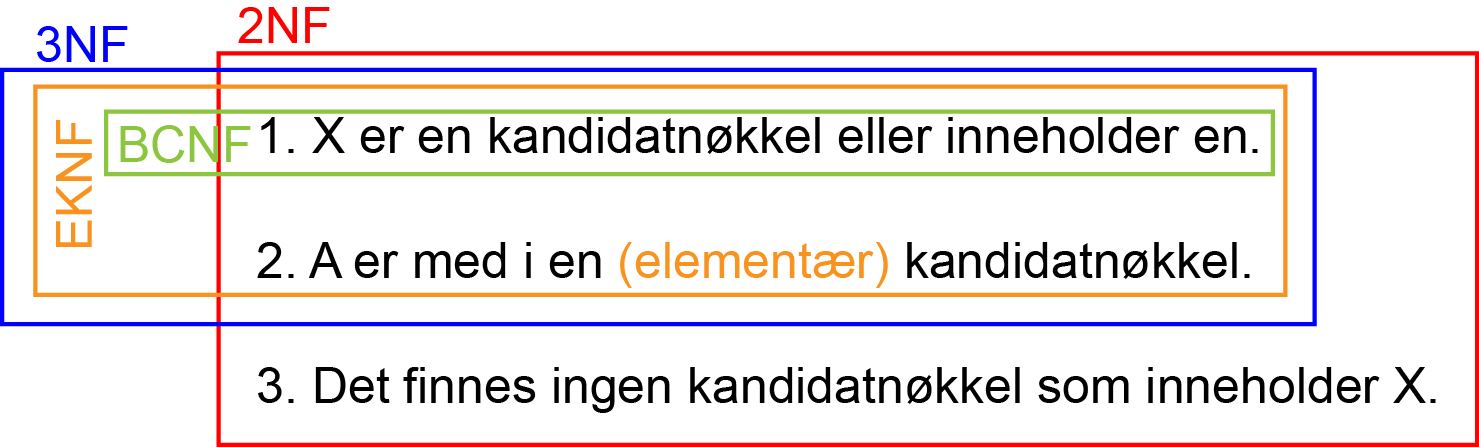
\includegraphics[width=\linewidth]{img/nfr.png}
	\caption{Regler for de forskjellige normalformene.}
\end{figure}

\subsection{Høyere Normalformer}
\subsubsection{4 NF}
Alle integritetsregler i form av FDer og MVDer. En relasjon $R$ er på 4NF hvis alle ikke-trivielle MVDer $X \twoheadrightarrow Y$ tilfredsstiller:
\begin{enumerate}
\item{$X$ er en supernøkkel i R.}
\end{enumerate}

\section{Flerverdiavhengigheter (MVD)}
Flerverdiavhengigheter brukes til å uttrykke integritetsregler utover FDer. 

MVDer oppstår når man plasserer to $n:n$-forhold i samme relasjon. Og for å uttrykke integritetsregler.

\paragraph{Eksempel} 
Gitt tabellen \textsf{Salg(pub, øltype, bryggeri)}. Regel: dersom en pub selger en øltype fra et bryggeri må den selge denne øltypen fra alle bryggeriene den forhandler med. 

Hvis da en pub selger pils fra Mack og fatøl fra Rignes. Må de også selge pils fra Rignes og fatøl fra Mack.
\begin{center}
\begin{tabular}{| l l l |}
\hline
pub & øltype & bryggeri\\
\hline
P1 & pils & Mack\\
P1 & fatøl & Rignes\\
P1 & pils & Rignes\\
P1 & fatøl & Mack\\
\hline
\end{tabular}
\end{center}

Tabellen påtvinges da flere tupler. 

$Y$ er fleravhengig av $X$, $Y \twoheadrightarrow X$. Hvis vi for enhver instans av $R$ har at hvis instansen inneholder to tupler $t_1$ og $t_2$ hvor $t_1[x] = t_2[x]$, så finnes også $u_1$ og $u_2$.

Hvis $Y \subseteq X$, så $X \twoheadrightarrow Y$, fordi:

\begin{center}
\begin{tabular}{| l  l  l |}
\hline
\multicolumn{2}{| c |}{X} &
\multicolumn{1}{| c |}{Z} \\
\hline
\multicolumn{1}{| c |}{W} &
\multicolumn{1}{| c |}{Y} &
\multicolumn{1}{| c |}{} \\
\hline
$w_1$ & $y_1$ & $z_1$ \\
$w_1$ & $y_1$ & $z_2$ \\
\hline
\end{tabular}
\end{center}

Alltid to tuple som er like i $x(w,y)$.

\paragraph{Trivielle MVDer} X $\twoheadrightarrow$ Y kalles triviell hvis og bare hvis vi enten har at Y $\subseteq$ X eller at XY er samtlige attributter i R.

\paragraph{Ekte MVDer}
En ikke-triviell X $\twoheadrightarrow$ Y, hvor X $\rightarrow$ Y \textit{ikke} holder, kalles en ekte MVD.

\section{Relasjonsalgebra}
Definerer en mengde av operasjoner på relasjoner. Gir oss et språk til å beskrive spørsmål om innholdet i relasjonene. Relasjonsalgebra er et \textbf{prosedyralt} spørrespråk -- sier \textit{hvordan} svaret skal beregnes.

\subsection{Algebra}
\begin{description}
\item[Domene] samling av verdier.
\item[Atomære operander] konstanter (representerer konkrete verdier i domenet) og variable (representerer vilkårlige verdier fra domenet).
\item[Operatorer] tar som argument operander og leverer som resultat en operand.
\item[Uttrykk] bygges av atomære operander med operatorer og parenteser.
\end{description}

\subsection{Mengdeoperatorer}
\begin{description}
\item[Union]: R $\cup$ S
\item[Snitt]: R $\cap$ S
\item[Differanse]: R $-$ S
\end{description}

R og S må ha identiske attributtmengder og identiske domener. Før operasjonen utføres, må S ordnes slik at attributtene kommer i samme rekkefølge som i R.

\begin{description}
\item[Eksempel på union]: \{a,b,c\} $\cup$ \{a,c,d\} = \{a,b,c,d\}
\item[Eksempel på snitt]: \{a,b,c\} $\cap$ \{a,c,d\} = \{a,c\}
\item[Eksempel på differanse]: \{a,b,c\} $-$ \{a,c,d\} = \{b\}
\end{description}

\subsection{Seleksjon}
$\sigma_C(R)$ er relasjonen som fås fra R ved å velge ut de tuplene i R som tilfredsstiller betingelsen C. C er et vilkårlig boolsk uttrykk bygget opp fra atomer på formen $op_1 \phi op_2$, der:
\begin{itemize}
\item{Operandene $op_1$ og $op_2$ er enten to attributter i R med samme domene, eller ett attributt i R og en konstant fra dette attributtets domene.}
\item{Operatoren $\phi \in \{=, \neq, <, >, \leq, \geq,$ \texttt{LIKE}\}.}
\end{itemize}

\subsection{Projeksjon}
$\pi_L(R)$ hvor R er en relasjon og L er en liste av attributter i R, er relasjonen som fås fra R ved å velge ut kolonnene til attributtene i L.
\begin{itemize}
\item{Relasjonen har et skjema med attributtene i L.}
\item{Ingen tupler skal forekomme flere ganger i $\pi_L(R)$.}
\end{itemize}

\subsection{Renavning}
$\rho_{S(A_1, A_2, \dots, A_n)}(R)$ renavner R til en relasjon med navn S og attributter $A_1, A_2, \dots, A_n$.
$\rho_S(R)$ renavner R til en relasjon med navn S. Attributtnavnene fra R beholdes.

\subsection{Kartetisk produkt}
$R \times S$ er relasjonen som fås fra R og S ved å danne alle mulige sammensetninger av ett tuppel fra R og ett tuppel fra S. Vi sier ofte at et tuppel $t$ fra R og et tuppel $u$ fra S blir \textbf{konkatenert} til et tuppel $v = tu$ i $R \times S$.

\subsection{Naturlig join}
$R \bowtie S$ er relasjonen som fås fra R og S ved å danne alle mulige sammensmeltinger av ett tuppel fra R med ett fra S der tuplene skal stemme overens i samtlige attributter med sammenfallende navn.
\begin{itemize}
\item{Fellesattributtene forekommer bare en gang i de sammensmeltede attributtene.}
\item{Resultatskjemaet har attributtene i R etterfulgt av de attributtene i S som ikke også forekommer i R.}
\end{itemize}

\subsubsection{Hengetuppel}
Et hengetuppel er et tuppel i en av relasjonene som ikke har noe matchende tuppel i den andre relasjonen. Dette får ingen representant i resultatrelasjonen etter en join.

\section{Indeksering}
En \textbf{indeks} på et attributt A er en datastruktur som gjør det lett å finne de elementene som har en bestemt verdi for A (\textbf{søkenøkkelen}). Indeksen er sortert på søkenøkkelen.

\subsection{Tette og tynne indekser}
En \textbf{tett} indeks har ett oppslag for hver verdi av søkenøkkelen. En \textbf{tynn} indeks har ett oppslag for hver datablokk.

\begin{center}
\begin{tabular}{| l | p{5cm} | p{5cm} |}
\hline
& \textbf{Tett} & \textbf{Tynn}\\
\hline
plass & ett indeksfelt pr. post & ett indeksfelt pr. datablokk\\ \hline
blokkaksesser & mange & få\\ \hline
postaksesser & direkte aksess & må lete innenfor blokken\\ \hline
exist-spørringer & bruker indeksen alene & må alltid aksessere blokken\\ \hline
bruk & overalt & ikke på uordnede elementer\\ \hline
endringer & må alltid oppdateres hvis postrekkefølgen endres & oppdateres bare hvis den første posten i en blokk endres\\
\hline
\end{tabular}
\end{center}

\subsection{Duplikate søkenøkler}
Ofte kalt clusterindekser. En klusterindeks kan brukes hvis filen er sortert selv om søkenøkkelen ikke er unik. Eksempel for tett indeks: ett indeksfelt pr. post. 

\subsection{Sekundærindekser}
Hvis filen er usortert, eller sortert på et annet attributt, kan man bruke en \textbf{sekundærindeks}. Denne er sortert på søkenøkkelen -- rakst søk. Første nivå er alltid tett -- høyere nivåer er tynne. Duplikater tillates.

\subsection{B$^+$-trær}
Hver node har $n$ søkenøkler og $n+1$ pekere. Indre noder: alle pekere er til subnoder. Løvnoder: $n$ datapekere og 1 nestepeker. Ingen noder kan være tomme.

Positive ting med B$^+$-trær er at antall nivåer er vanligvis veldig lavt -- typisk 3. Intervallsøking går veldig raskt. Ved stor $n$ er det sjelden nødvendig å splitte/slå sammen noder. Disk I/O kan reduseres ved å holde indeksblokkene i minnet. Et minus med slike trær kan være at et søk må alltid gå fra roten til en løvnode. Dvs. antall blokkaksesser er lik høyden på treet pluss aksessering av selve postene.

\subsection{Hashtabeller}
Bruker en hashfunksjon fra søkenøkkelen til en arrayindeks med peker videre til hvilken bøtte (bucket) som eventuelt inneholder den aktuelle posten.

Positive sider ved dette er at man får signifikant færre diskoperasjoner enn med vanlige indekser og B-trær. Også raskt søk etter spesifikk søkenøkkel. Negative sider med hashtabeller kan være at flere poster kan føre til flere blokker per bucket. Og dårlig den er dårlig på intervallsøk.

\subsection{Indekser i SQL}
\subsubsection{Syntaks}
\begin{lstlisting}
CREATE INDEX name ON relation_name (attribute)
CREATE UNIQUE INDEX name ON relation_name (attribute)
DROP INDEX name
\end{lstlisting}

Linje nr. 2 definerer en kandidatnøkkel. Man kan ikke angi type indeks, f.eks. B-tre, hash osv. Og man kan ikke angi parametere som loadfaktor, hashstørrelse osv.

\subsubsection{Spørringer med flere betingelser}
\begin{lstlisting}
SELECT ... FROM R WHERE a = 30 AND b < 5
\end{lstlisting}

Strategi: bruk en indeks, f.eks på a. Finn og \textit{hent} alle postene med a = 30. Søk gjennom disse postene for å finne dem med b $<$ 5.

\section{Systemfeil og logging}
Vi ønsker at data alltid skal være riktige og nøyaktige. Eksempel på tvilsomme data kan være: (Hansen er 51, Lie er 48, Olsen er 61).
\begin{center}
\textsf{Ansatt}
\begin{tabular}{|l | l|}
\hline
Navn & Alder\\ \hline
Hansen & 56 \\ \hline
Lie & 2489\\ \hline
Olsen & 1\\ \hline
\end{tabular}
\end{center}

\subsection{Integritetsregler og konsistens}
\Intt er predikater som data må tilfredsstille. Eksempel: $X \rightarrow Y$ holder i R.

\paragraph{Def. av konsistens}
Konsistent tilstand: tilfredsstiller alle (statiske) \intt.
Konsistent database: databasen er i en konsistent tilstand.

\subsection{Transaksjoner}
En \textbf{transaksjon} er en samling aksjoner som bevarer konsistens. 
\paragraph{En viktig antagelse} Hvis T starter i en konsistent tilstand, og T eksekverer alene, så vil T avslutte med å etterlate databasen i en kosistent tilstand.

\subsection{Klassifikasjon av hendelser}

% Set the overall layout of the tree
\tikzstyle{level 1}=[level distance=2.5cm, sibling distance=2.5cm]
\tikzstyle{level 2}=[level distance=2.5cm, sibling distance=1cm]

% Define styles for bags and leafs
\tikzstyle{bag} = [text width=4em, text centered]
\tikzstyle{end} = [circle, minimum width=3pt,fill, inner sep=0pt]

\begin{tikzpicture}[grow=right, sloped]
\node[bag] {Hendelser}
    child {
        node {Ønskede}        
    }
    child {
        node[bag] {Uønskede}        
        child {
                node[end, label=right:
                    {Forventede}] {}
                edge from parent
                node[above] {}
                node[below]  {}
            }
            child {
                node[end, label=right:
                    {Uventede}] {}
                edge from parent
                node[above] {}
                node[below]  {}
            }
    };
\end{tikzpicture}

\subsection{Transaksjonsoperasjoner}
\begin{description}
\item[input(x)] diskblokk med x $\rightarrow$ primærminnet.
\item[read(x,v)] verdien av x i blokken $\rightarrow$ v.
\item[write(x,v)] v $\rightarrow$ verdien av x i blokken.
\item[output(x)] minneblokk med x $\rightarrow$ disk.
\end{description}

\paragraph{En viktig antakelse} I beskrivelsen av operasjonene har vi implisitt antatt at hvert dataelement ligger i en diskblokk/minneblokk. Dette er opplagt riktig hvis dataelementet er en blokk.

\subsection{Ufullførte transaksjoner}
Dette er hovedproblemet i transaksjonshåndtering. Eksempel med \inttt: A = B.
\begin{center}
\begin{tabular}{ll}
T1: & $A \leftarrow A \times 2$\\
& $B \leftarrow B \times 2$\\
\end{tabular}
\end{center}

\begin{center}
\begin{tabular}{lll}
T1: & read(A,t); & $t \leftarrow t \times 2;$\\
& write(A,t); &\\
& read(B,t); & $t \leftarrow t \times 2;$\\
& write(B,t); &\\
& output(A);&\\
&&\textbf{\textcolor{red}{Her skjer feilen.}}\\
&output(B);&\\
\end{tabular}
\end{center}

I primærminnet vil både A og B være 16 etter transaksjonen, men på disk er A satt til 16 og B til 8.
Transaksjoner må være \textbf{atomære}. Dette gir oss to muligheter:
\begin{enumerate}
\item{Å utføre alle operasjonene i transaksjoner, eller}
\item{å ikke utføre noen av operasjonene i transaksjonen.}
\end{enumerate}

\subsection{Logging}

\section{Transaksjonshåndtering}
En \textbf{transaksjon} er en \textit{sekvens} av operasjoner som \textit{bevarer konsistens} i databasen.

\paragraph{ACID-egenskapene}
\begin{description}
\item[Atomicity] enten blir hele transaksjonen utført eller så blir ikke noe av den utført.
\item[Consistency] transaksjoner skal bevare konsistens.
\item[Isolation] transaksjoner skal ikke merke at andre transaksjoner utføres samtidig med dem selv.
\item[Durability] når tansaksjoner er avsluttet, skal effekten av dem være varig og ikke kunne påvirkes av systemfeil.
\end{description}

\subsection{Eksekveringsplaner}
En \textbf{eksekveringsplan} S for en mengde transaksjoner $\{T_1, \dots, T_n\}$ er en \textit{fletting} av operasjonene i $\{T_1, \dots, T_n\}$.

Egenskaper hos S:
\begin{itemize}
\item{Hvert element i S er en operasjon i nøyaktig en av transaksjonene.}
\item{Hver operasjon i en transaksjon er element i S nøyaktig en gang.}
\item{S bevarer rekkefølgen på operasjonene fra hver enkelt transaksjon.}
\end{itemize}

\paragraph{Transaksjonseksempel}
Integritetsregel: A = B

\begin{center}
\begin{tabular}{l l l l}
T1: & read(A); & T2: & read(A);\\
& A $\leftarrow$ A+100; &  & A $\leftarrow$ A $\times$2;\\
& write(A); & & write(A);\\
& read(B); & & read(B);\\
& B $\leftarrow$ B+100; && B $\leftarrow$ B $\times$2;\\
& write(B); && write(B);\\
\end{tabular}
\end{center}

\paragraph{Eksikveringsplan}
\begin{center}
\begin{tabular}{l l | l | l}
& & A & B\\
T1 & T2 & \textcolor{blue}{25} & \textcolor{blue}{25}\\
\hline
read(A); A $\leftarrow$ A+100; & & &\\
write(A); & & 125 &\\
read(B); B $\leftarrow$ B+100; & & &\\
write(B); & & & 125\\
& read(A); A $\leftarrow$ A $\times$2; & &\\
& write(A); & 250 &\\
& read(B); B $\leftarrow$ B $\times$2; & &\\
& write(B); & & 250\\
& & \textcolor{blue}{250} & \textcolor{blue}{250}\\
\end{tabular}
\end{center}

Dette er en \textit{serielle} eksikveringsplan, tar en transaksjon om gangen.

Man vil ha eksikveringsplaner som er gode. Begrepet god skal være uavhengig av initialtilstanden og transaksjonssemantikken. Begrepet skal også bare være avhening av lese- og skriveoperasjonene og deres innbyrdes rekkefølge.

\subsubsection{Noen begreper}
\begin{description}
\item[Transaksjon] En sekvens av leseoperasjoner $r_i(A)$ og skriveoperasjoner $w_i(B)$.
\item[Eksekveringsplan] For transaksjonene $\{T_1, \dots, T_n\}$: en fletting av $T_1, \dots, T_n$.
\item[Seriell eksikveringsplan] Plan hvor alle operasjonene i en transaksjon fullføres før neste transaksjon startes.
\item[Konflikt i en eksikveringsplan] 
	\begin{enumerate}
	\item{\textbf{Lese-skrive-konflikt:} et par av operasjonene av formen $\dots r_i(A) \dots w_k(A) \dots$ eller $\dots w_i(A) \dots r_k(A) \dots$, hvor i $\neq$ k.}
	\item{\textbf{Skrive-skrive-konflikt:} et par av operasjoner av formen $\dots w_i(A) \dots w_k(A) \dots$, hvor i $\neq$ k.}
	\item{\textbf{Intratransaksjonskonflikt:} Et par av operasjoner av formen $\dots o_i(A) \dots o_i(B) \dots$, hvor $o_i$ er $w_i$ eller $r_i$.}
	\end{enumerate}
\end{description}

\subsection{Konfliktserialiserbarhet}
To eksikveringsplaner $S_1$ og $S_2$ kalles \textbf{konfliktekvivalente} hvis $S_1$ kan omformes til $S_2$ ved en serie ombyttinger av nabooperasjoner som ikke er i konflikt med hverandre. En eksikveringsplan er \textbf{konfliktserialiserbar} hvis den er konfliktekvivalent med en seriell eksekveringsplan.

\subsubsection{En dårlig eksikveringsplan} 
$S_D = r_1(A);\textcolor{red}{w_1(A);r_2(A);}w_2(A);r_2(B);\textcolor{red}{w_2(B);r_1(B);}w_1(B);$

Her har vi en konflikt mellom $w_2(B)$ og $r_1(B)$. Disse kan ikke bytte plass, så $S_D$ kan ikke være konfliktekvivalent med den serielle planen $T_1;T_2$. Vi har også en konflikt mellom $w_1(A)$ og $r_2(A)$ som følgelig heller ikke kan bytte plass. Dermed kan $S_D$ heller ikek være konfliktekvivalent med den serielle planen $T_2;T_1$. $S_D$ er altså ikke konfliktserialiserbar.




\end{document}
